\documentclass[leqno]{article}
% Shared mark scheme preamble for resources.danieljsmith.org: the pack
% preamble, unchanged, then the scheme's own layer. A scheme's .tex is
% rendered from its YAML (scripts/README.md, Mark schemes), never edited.
\input{\CurrentFilePath/pack_preamble.tex}

% The page: equal side margins, so the table runs the full width of the
% header rule. The footers' right edge follows the text's.
\geometry{left=0.8in, right=0.8in}
\makeatletter
\renewcommand{\djs@footR}[1]{%
  \put(\dimexpr1in+\hoffset+\oddsidemargin+\textwidth\relax,
    -\dimexpr\paperheight-0.32in\relax){\makebox[0pt][r]{#1}}}
\makeatother

\usepackage[export]{adjustbox}
\usepackage{tabularray}
\definecolor{msGrid}{RGB}{176, 172, 164}
\definecolor{msTint}{RGB}{245, 243, 239}

% The header on every page, the front page included, and the booklet label
% under the contents-page title. \djsQuestionPageStyle stays empty.
\newcommand{\djsSchemeHeader}[1]{%
  \djsPackHeader[markscheme]{\textit{Mark scheme} - #1}%
  \renewcommand{\djsPackTitle}{#1}%
  \renewcommand{\djsBookletLabel}{Mark scheme}%
}

% The front page: the contents heading, spaced as tocloft spaces the packs'
% "Questions", then the contents table. A question's name and page number
% both link to its first page.
\newcommand{\msContentsHeading}{%
  \vskip\cftbeforetoctitleskip
  {\noindent\cfttoctitlefont\contentsname\par}%
  \vskip\cftaftertoctitleskip}
\NewTblrEnviron{mscontents}
\SetTblrInner[mscontents]{
  colspec = {Q[wd=26mm, l] X[l] Q[wd=16mm, c] Q[wd=14mm, r]},
  width = \linewidth,
  rowsep = 4pt, colsep = 6pt,
  hlines = {0.4pt, msGrid}, vlines = {0.4pt, msGrid},
  hline{2} = {2.2pt, scarlet},
  row{1} = {font=\small\bfseries},
  row{Z} = {font=\bfseries},
  column{2} = {font=\small},
}
\newcommand{\msContentsQuestion}[1]{\hyperref[q:#1]{Question #1}}
\newcommand{\msContentsPage}[1]{\hyperref[q:#1]{\pageref*{q:#1}}}
\newcommand{\msSep}{\hspace{0.9em}}

% The conventions pages' layout: headings in the documents' own bold, tables
% ruled and padded as the scheme's, roomy lists.
\newcommand{\msHead}[1]{%
  \par\vspace{18pt}%
  {\noindent\bfseries #1\par}%
  \vspace{6pt}}
\NewTblrEnviron{mstblr}
\SetTblrInner[mstblr]{rowsep = 6pt, colsep = 6pt,
  hlines = {0.4pt, msGrid}, vlines = {0.4pt, msGrid}}
\newenvironment{msList}
  {\begin{itemize}[leftmargin=1.2em, itemsep=5pt, topsep=3pt, parsep=0pt]}
  {\end{itemize}}

% A question's first page: the link target and the PDF bookmark, as
% \questionitem gives the packs.
\newcommand{\msQnum}{}
\newcommand{\msQuestion}[1]{%
  \clearpage
  \renewcommand{\msQnum}{#1}%
  \phantomsection\label{q:#1}%
  \addcontentsline{toc}{subsection}{\protect\djsTocEntry{#1}}}

% The scheme's table: Question 16mm, Scheme the rest, Marks 16mm, Notes
% 44mm; every cell ruled in msGrid; the scarlet rule under the head row. A
% long table has no caption or "continued" foot; a continuation page opens
% with a muted line above the repeated head row. The rules across a part's
% rows, the alternative's tint and the total row are the rendered table's.
\NewTblrTheme{ms}{%
  \DefTblrTemplate{firsthead}{default}{}%
  \DefTblrTemplate{middlehead,lasthead}{default}{%
    {\small\itshape\color{djsMuted}Question \msQnum\ continued\par}%
    \vspace{6pt}}%
  \DefTblrTemplate{firstfoot,middlefoot,lastfoot}{default}{}%
}
\NewTblrEnviron{msscheme}
\SetTblrOuter[msscheme]{long, theme=ms, entry=none, label=none}
\SetTblrInner[msscheme]{
  colspec = {Q[wd=16mm, l] X[l] Q[wd=16mm, c] Q[wd=44mm, l]},
  width = \linewidth,
  rowsep = 6pt, colsep = 6pt,
  rowhead = 1,
  vlines = {0.4pt, msGrid},
  hline{1} = {0.4pt, msGrid}, hline{2} = {2.2pt, scarlet},
  hline{Z} = {0.4pt, msGrid},
  column{1} = {font=\bfseries}, column{3} = {font=\bfseries},
  column{4} = {font=\small},
  row{1} = {rowsep=4pt, font=\small\bfseries},
}

% Two marks on a row: each note starts with its code.
\newcommand{\msNote}[2]{\textbf{#1}\enspace #2}
% A full-row figure: the worked solution's own picture, scaled uniformly and
% only down, to the table less the Question column. The picture is drawn
% with the line width it has in the solutions document, at its list depth
% there (the optional argument, 1 by default: a part's working), so one
% sized by \linewidth keeps its size; tabularray sets the cell's \linewidth
% to the cell's measured width, which would shrink it at every pass. The
% widths are measured once, in a solution box at the packs' text width
% (pack_preamble.tex's margins, 0.8in and 1in).
\newlength{\msSpanW}
\makeatletter
\newcommand{\ms@keepLW}[1]{%
  \expandafter\xdef\csname ms@solnLW@#1\endcsname{\the\linewidth}}
\AtBeginDocument{%
  \setlength{\msSpanW}{\dimexpr\textwidth-16mm-28pt\relax}%
  \setbox\z@\vbox{%
    \begin{minipage}{\dimexpr\paperwidth-1.8in\relax}
      \begin{djsSolution}
        \ms@keepLW{0}%
        \begin{enumerate}\item \ms@keepLW{1}%
        \begin{enumerate}\item \ms@keepLW{2}%
        \begin{enumerate}\item \ms@keepLW{3}%
        \end{enumerate}\end{enumerate}\end{enumerate}
      \end{djsSolution}
    \end{minipage}}}
\newcommand{\msFigure}[2][1]{%
  \adjustbox{max width=\msSpanW, max totalheight=0.6\textheight, valign=t}{%
    \hsize=\csname ms@solnLW@#1\endcsname
    \linewidth=\hsize
    #2}}
\makeatother
% A figure mark's feature, in the Scheme column.
\newcommand{\msFeature}[1]{\textit{#1}}
% An alternative's title row.
\newcommand{\msAlternative}[1]{\textit{Alternative:} #1}
% Drafts only: a queried mark's code, the query's why under its note, and a
% flag in its part's place.
\newcommand{\msQueried}[2]{#1~\(\to\) #2?}
\newcommand{\msQuery}[1]{{\itshape\color{djsMuted}Query: #1}}
\newcommand{\msFlag}[2]{\textbf{#1:}\enspace #2}


\djsSchemeHeader{Hyperbolic Functions}
\djsSitePath{Core Pure}{Miscellaneous Pure}

\djsLastUpdated{24 October 2026}
\begin{document}
\djsSetQuestionCount{18}
\djsAddMarks{1}{4}
\djsAddMarks{2}{7}
\djsAddMarks{3}{7}
\djsAddMarks{4}{6}
\djsAddMarks{5}{8}
\djsAddMarks{6}{6}
\djsAddMarks{7}{8}
\djsAddMarks{8}{12}
\djsAddMarks{9}{11}
\djsAddMarks{10}{5}
\djsAddMarks{11}{9}
\djsAddMarks{12}{12}
\djsAddMarks{13}{8}
\djsAddMarks{14}{14}
\djsAddMarks{15}{10}
\djsAddMarks{16}{8}
\djsAddMarks{17}{10}
\djsAddMarks{18}{14}
\vspace*{6pt}
\djsContentsTitle
\vspace{30pt}
\msContentsHeading
\begin{mscontents}{}
Question & Marks by part & Marks & Page \\
\msContentsQuestion{1} & & 4 & \msContentsPage{1} \\
\msContentsQuestion{2} & (a)\,2\msSep (b)\,5 & 7 & \msContentsPage{2} \\
\msContentsQuestion{3} & (a)\,3\msSep (b)\,4 & 7 & \msContentsPage{3} \\
\msContentsQuestion{4} & (a)\,2\msSep (b)(i)\,1\msSep (b)(ii)\,3 & 6 & \msContentsPage{4} \\
\msContentsQuestion{5} & (a)\,4\msSep (b)\,4 & 8 & \msContentsPage{5} \\
\msContentsQuestion{6} & (a)\,2\msSep (b)\,4 & 6 & \msContentsPage{6} \\
\msContentsQuestion{7} & (a)\,5\msSep (b)\,3 & 8 & \msContentsPage{7} \\
\msContentsQuestion{8} & (a)\,2\msSep (b)(i)\,2\msSep (b)(ii)\,3\msSep (c)\,3\msSep (d)\,2 & 12 & \msContentsPage{8} \\
\msContentsQuestion{9} & (a)\,4\msSep (b)\,3\msSep (c)\,4 & 11 & \msContentsPage{9} \\
\msContentsQuestion{10} & & 5 & \msContentsPage{10} \\
\msContentsQuestion{11} & (a)\,5\msSep (b)\,4 & 9 & \msContentsPage{11} \\
\msContentsQuestion{12} & (a)(i)\,4\msSep (a)(ii)\,2\msSep (b)\,6 & 12 & \msContentsPage{12} \\
\msContentsQuestion{13} & (a)\,4\msSep (b)\,4 & 8 & \msContentsPage{13} \\
\msContentsQuestion{14} & (a)\,2\msSep (b)\,5\msSep (c)(i)\,2\msSep (c)(ii)\,5 & 14 & \msContentsPage{14} \\
\msContentsQuestion{15} & (a)\,3\msSep (b)\,3\msSep (c)\,4 & 10 & \msContentsPage{15} \\
\msContentsQuestion{16} & (a)\,4\msSep (b)\,4 & 8 & \msContentsPage{16} \\
\msContentsQuestion{17} & (i)\,4\msSep (ii)\,2\msSep (iii)\,4 & 10 & \msContentsPage{17} \\
\msContentsQuestion{18} & (a)\,4\msSep (b)\,2\msSep (c)\,2\msSep (d)\,6 & 14 & \msContentsPage{18} \\
\SetCell[c=2]{r} Total & & 159 & \\
\end{mscontents}
\newpage
% The conventions pages, shared by every pack's mark scheme: one source of
% truth, \input after the front page, with no strand or pack logic. The keys
% on the first side, the rules on the second. The scheme layer defines
% \msHead, msList and mstblr.
\vspace*{6pt}%
{\noindent\cfttoctitlefont Reading the mark scheme\par}%
\vspace{10pt}%
These rules apply throughout, unless a note says otherwise.

\msHead{Marks}
Every mark is worth one, so \textbf{M1 A1} on a row is two marks. Only marks
coded ft follow through.\par
\vspace{10pt}%
\begin{mstblr}{
  colspec = {Q[wd=15mm, l] X[l]},
  width = \linewidth,
  hline{2} = {2.2pt, scarlet},
  column{1} = {font=\bfseries},
  row{1} = {font=\small\bfseries, rowsep=4pt},
}
Code & Meaning \\
M1 & Method: a correct method, applied to this question. A slip doesn't cost it if the method is clear. A formula must be used, not just quoted. \\
dM1 & Dependent method: as M1, but only if the method mark before it was earned, unless its note names another. \\
A1 & Accuracy: a correct answer or step. It needs the method mark it follows. \\
A1ft & As A1, following through from an earlier answer that the note names. \\
A1~AG & The last mark of a part whose answer is printed in the question: complete working, with no errors. \\
B1 & A correct value, fact or statement. It needs no method mark. \\
B1ft & As B1, following through from an earlier answer that the note names. \\
E1 & A written explanation, interpretation or conclusion. Concluding a proof by induction needs every earlier mark. \\
\end{mstblr}

\msHead{Abbreviations}
ft and AG qualify a code in the Marks column. The others appear in the
notes.\par
\vspace{10pt}%
\begin{mstblr}{
  colspec = {Q[wd=17mm, l] X[l] Q[wd=15mm, l] X[l]},
  width = \linewidth,
  column{1} = {font=\bfseries}, column{3} = {font=\bfseries},
}
ft & follow through & AG & answer given in the question \\
cao & correct answer only, with no follow-through & cso & correct solution only: no errors in the part \\
oe & or an equivalent form & awrt & any answer that rounds to this value \\
soi & seen, or implied by later working & isw & ignore working after a correct answer \\
SC & special case: credit outside the main method & their & the student's own earlier value \\
condone & a slip that doesn't cost the mark & [\;\,] & working the mark doesn't need \\
s.f. & significant figures & d.p. & decimal places \\
\end{mstblr}

\newpage
\msHead{Reading the scheme}
\begin{msList}
\item Each row is a line of working, with the marks it earns beside it.
  Where a row carries two marks, each note starts with its code.
\item \textbf{[\textit{n}]} ends each part with its total.
\item A shaded \textit{Alternative} is a second method for the same total.
  Mark an answer by the method it follows.
\item Any other valid method earns the equivalent marks, unless the question
  names a method or says \textit{hence}.
\item A sketch earns one B1 for each feature named below its figure.
\end{msList}

\msHead{Accuracy and answers}
\begin{msList}
\item Unless a question says otherwise, give answers to 3 significant
  figures, and angles in degrees to 1 decimal place. Angles in radians take
  3 significant figures.
\item A final answer with more figures is accepted if it rounds to the
  scheme's value; one with fewer is not. An answer spoiled by rounding too
  early loses its accuracy mark.
\item Where a question asks for an exact answer, a decimal loses the final
  accuracy mark. Otherwise either is accepted.
\item Wrong or missing units cost nothing unless the question asks for them.
\item A correct answer with no working earns full marks, unless the question
  needs the working: show that, prove, hence, a method it names, or an exact
  answer. A wrong answer with no working earns nothing. Calculator answers
  are treated the same way.
\item A correct answer, once reached, isn't spoiled by later working (isw).
\end{msList}

\msHead{Value of $\boldsymbol{g}$}
\begin{msList}
\item Take $g = 9.8\,\mathrm{m\,s^{-2}}$ unless a question states a value,
  which is then the only one accepted. Answers that use $g = 9.8$ may be
  given to 2 or 3 significant figures.
\item Where a question doesn't state $g$, an answer worked with $g = 10$
  throughout earns the same marks, keeping any value printed in the
  question. The worked solutions list the final answers with $g = 10$.
\end{msList}


\msQuestion{1}
\begin{msscheme}{
  hline{3-5} = {2-Z}{0.4pt, msGrid},
  hline{6} = {0.4pt, msGrid},
  row{6} = {font=\bfseries},
}
Question & Scheme & Marks & Notes \\
1 & {\(2\left(\frac{e^x-e^{-x}}{2}\right)+5\left(\frac{e^x+e^{-x}}{2}\right)=6\)\\[4pt] \(\Rightarrow \ldots e^{2x}+\ldots e^x+\ldots=0\)} & M1 & {Substitutes both exponential forms and multiplies through by a multiple of \(e^x\) to reach a three-term quadratic in \(e^x\). Condone sign and coefficient slips.} \\
& {\(7e^{2x}-12e^x+3=0\)} & A1 & {oe, any multiple or arrangement, such as \(7e^{2x}+3=12e^x\).} \\
& {\(e^x=\frac{6\pm\sqrt{15}}{7}\Rightarrow x=\ln(\ldots)\)} & M1 & {Solves their three-term quadratic in \(e^x\) by formula, completing the square, factorising or calculator, and takes ln of at least one positive root.} \\
& {\(x=\ln\left(\frac{6+\sqrt{15}}{7}\right),\ x=\ln\left(\frac{6-\sqrt{15}}{7}\right)\)} & A1 & {cso. Both, in any exact log form such as \(\ln(6\pm\sqrt{15})-\ln 7\). A0 if either is rejected.} \\
\nopagebreak \SetCell[c=2]{r} Total for Question 1 & & 4 & \\
\end{msscheme}

\msQuestion{2}
\begin{msscheme}{
  hline{3-4,6-10} = {2-Z}{0.4pt, msGrid},
  hline{5,11} = {0.4pt, msGrid},
  row{11} = {font=\bfseries},
}
Question & Scheme & Marks & Notes \\
2(a) & {\(\tanh x = \dfrac{\frac12(e^x - e^{-x})}{\frac12(e^x + e^{-x})}\)\\[4pt] \(\phantom{\tanh x} = \dfrac{(e^x - e^{-x})e^x}{(e^x + e^{-x})e^x}\)} & M1 & {Writes \(\sinh x/\cosh x\) using both exponential definitions and multiplies numerator and denominator by \(e^x\); or divides the printed fraction through by \(e^x\).} \\
& {\(\phantom{\tanh x} = \dfrac{e^{2x}-1}{e^{2x}+1}\)} & A1~AG & {Correct definitions leading without error to the printed result; combined steps accepted.} \\
\nopagebreak & & [2] & \\
2(b) & {\(\dfrac{e^{2(x-\ln 2)}-1}{e^{2(x-\ln 2)}+1} = \dfrac37\)\\[4pt] \(\Rightarrow e^{2(x-\ln 2)} = \ldots\)} & M1 & {Substitutes \(x-\ln 2\), or a defined variable for it, into the result of (a), sets it equal to \(\frac37\) and rearranges for the exponential. Condone sign slips.} \\
& {\(e^{2(x-\ln 2)} = \tfrac52\)} & A1 & {oe, such as \(e^{2x} = 10\), or \(e^{2y} = \frac52\) with \(y = x - \ln 2\).} \\
& {\(2(x-\ln 2) = \ln \text{"}\tfrac52\text{"}\)} & M1 & {Takes ln of both sides of their \(e^{2(x-\ln 2)} = c\), \(c > 0\), giving a linear equation in \(x\).} \\
& {\(2x = \ln \text{"}\tfrac52\text{"} + \ln 4 = \ln(\ldots)\)} & dM1 & {Uses \(2\ln 2 = \ln 4\) and \(\ln a + \ln b = \ln ab\) to reach a single log; or \(e^{-2\ln 2} = \frac14\) before taking logs.} \\
& {\(x = \tfrac12 \ln 10\)} & A1 & {cso. \(x = \frac12\ln 10\) or \(k = 10\); \(\ln\sqrt{10}\) or a decimal scores A0.} \\
\nopagebreak & & [5] & \\
\nopagebreak \SetCell[c=2]{r} Total for Question 2 & & 7 & \\
\end{msscheme}

\msQuestion{3}
\begin{msscheme}{
  hline{3-5,7-10} = {2-Z}{0.4pt, msGrid},
  hline{6,11} = {0.4pt, msGrid},
  row{11} = {font=\bfseries},
}
Question & Scheme & Marks & Notes \\
3(a) & {\(\cosh x + \sinh x = \frac{(e^x+e^{-x})+(e^x-e^{-x})}{2}\)} & M1 & {Substitutes both exponential definitions into either expression and combines over 2. Condone sign slips.} \\
& {\(\phantom{\cosh x + \sinh x} = \frac{2e^x}{2} = e^x\)} & A1 & {Correct combined numerator simplified to \(e^x\) without error.} \\
& {\(\cosh x - \sinh x = \frac{(e^x+e^{-x})-(e^x-e^{-x})}{2}\)\\[4pt] \(\phantom{\cosh x - \sinh x} = \frac{2e^{-x}}{2} = e^{-x}\)} & A1~AG & {Correct substituted expression with the subtraction applied to both terms of \(\sinh x\), leading without error to \(e^{-x}\).} \\
\nopagebreak & & [3] & \\
3(b) & {\(2(e^x+e^{-x}) - \tfrac32(e^x-e^{-x}) = 5\)\\[4pt] \(\Rightarrow \ldots e^{2x} + \ldots e^x + \ldots = 0\)} & M1 & {Substitutes exponential forms, or uses (a), and multiplies by \(e^x\) to reach a three-term quadratic in \(e^x\). Condone sign and coefficient slips.} \\
& {\(e^{2x} - 10e^x + 7 = 0\)} & A1 & {oe, any multiple, terms in any order, or in a substituted letter for \(e^x\).} \\
& {\(e^x = \frac{10 \pm \sqrt{72}}{2} \Rightarrow x = \ln(\ldots)\)} & M1 & {Solves their three-term quadratic in \(e^x\) by any means, calculator allowed, and takes ln of at least one positive root.} \\
& {\(x = \ln(5+3\sqrt2)\) or \(x = \ln(5-3\sqrt2)\)} & A1 & {Both exact, and no others. Accept equivalent exact forms, such as \(\ln\frac{10\pm\sqrt{72}}{2}\), or \(\ln 7-\ln(5+3\sqrt2)\) for the second.} \\
\nopagebreak & & [4] & \\
\nopagebreak \SetCell[c=2]{r} Total for Question 3 & & 7 & \\
\end{msscheme}

\msQuestion{4}
\begin{msscheme}{
  hline{3-4,6,8-10} = {2-Z}{0.4pt, msGrid},
  hline{5,7,11} = {0.4pt, msGrid},
  row{11} = {font=\bfseries},
}
Question & Scheme & Marks & Notes \\
4(a) & {\(\operatorname{sech} 2x = \dfrac{1}{2\cosh^2 x - 1}\)\\[4pt] \(\phantom{\operatorname{sech} 2x} = \dfrac{1}{\frac{2}{\operatorname{sech}^2 x} - 1}\)} & M1 & {Takes the reciprocal of the identity and replaces \(\cosh^2 x\) by \(\frac{1}{\operatorname{sech}^2 x}\), or substitutes \(\operatorname{sech}^2 x = \frac{1}{\cosh^2 x}\) into the RHS.} \\
& {\(\phantom{\operatorname{sech} 2x} = \dfrac{\operatorname{sech}^2 x}{2 - \operatorname{sech}^2 x}\)} & A1~AG & {Printed result reached without error from a correct substituted expression; combined simplification accepted. Working from the RHS must end at \(\frac{1}{\cosh 2x}\) via the identity.} \\
\nopagebreak & & [2] & \\
4(b)(i) & {\(0 < f(x) < 1\)} & B1 & {oe, such as \((0, 1)\). B0 if either bound is included.} \\
\nopagebreak & & [1] & \\
4(b)(ii) & {\(\operatorname{sech} 2x = \dfrac{\operatorname{sech}^2 x}{2 - \operatorname{sech}^2 x}\)\\[4pt] \(0 < \operatorname{sech} x < 1 \Rightarrow 2 - \operatorname{sech}^2 x > 1\)} & M1 & {Uses (a) with \(0 < \operatorname{sech} x < 1\) to bound the denominator or the fraction, such as \(2 - \operatorname{sech}^2 x > 1\).} \\
& {\(\Rightarrow \operatorname{sech} 2x < \operatorname{sech}^2 x\)} & A1 & \\
& {\(0 < \operatorname{sech} x < 1 \Rightarrow \operatorname{sech}^2 x < \operatorname{sech} x\)\\[4pt] \(\Rightarrow \operatorname{sech} 2x < \operatorname{sech} x\)} & A1~AG & {Justifies \(\operatorname{sech}^2 x < \operatorname{sech} x\) from \(0 < \operatorname{sech} x < 1\) and concludes the printed inequality. A0 if that justification is missing.} \\
\nopagebreak & & [3] & \\
\nopagebreak \SetCell[c=2]{r} Total for Question 4 & & 6 & \\
\end{msscheme}

\msQuestion{5}
\begin{msscheme}{
  hline{3-7,9-12} = {2-Z}{0.4pt, msGrid},
  hline{8,13} = {0.4pt, msGrid},
  row{13} = {font=\bfseries},
}
Question & Scheme & Marks & Notes \\
5(a) & \SetCell[c=3]{c} \msFigure{\begin{tikzpicture}
\begin{axis}[
    axis lines=middle,
    xlabel={$x$},
    ylabel={$y$},
    xmin=-1.2, xmax=1.2,
    ymin=-5, ymax=9.5,
    width=0.78\linewidth,
    height=10cm,
    samples=300,
    clip=false,
    xtick={0},
    ytick={-2},
    tick label style={font=\small},
    label style={font=\small},
    every axis plot/.append style={thick}
]
\addplot[domain=-1.2:1.2] {exp(2*x)+exp(-2*x)-2};
\addplot[domain=-0.23:1.2] {3-5*exp(-2*x)};
\addplot[dashed, domain=-1.2:1.18, samples=2] {3};
\node[fill=white, inner sep=1pt] at (axis cs:0.93,5.9) {$C_1$};
\node[fill=white, inner sep=1pt] at (axis cs:0.90,1.7) {$C_2$};
\node[fill=white, inner sep=1pt] at (axis cs:-0.3,3.45) {$y=3$};
\end{axis}
\end{tikzpicture}} & & \\
& \msFeature{Shape} & B1 & {\(C_1\): U shape symmetric about the \(y\)-axis, minimum at the origin, meeting the axes only there.} \\
& \msFeature{Shape} & B1 & {\(C_2\): increasing curve, approaching its asymptote from below as \(x\to\infty\), unbounded below as \(x\to-\infty\).} \\
& \msFeature{Asymptotes} & B1 & {\(y=3\) stated as the asymptote of \(C_2\); none drawn for \(C_1\).} \\
& \msFeature{Intercepts} & B1 & {\((0,-2)\) and \(\left(\frac12\ln\frac53,0\right)\) oe, or awrt 0.255 for the \(x\)-intercept.} \\
\nopagebreak & & [4] & \\
5(b) & {\(e^{2x}+e^{-2x}-2=3-5e^{-2x}\)} & M1 & {Replaces \(\cosh 2x\) by \(\frac12(e^{2x}+e^{-2x})\) and multiplies through to reach a three-term quadratic in \(e^{2x}\). Condone sign and coefficient slips.} \\
& {\(e^{4x}-5e^{2x}+6=0\)} & A1 & {oe, in \(e^{2x}\) or a substituted variable.} \\
& {\((e^{2x}-2)(e^{2x}-3)=0\)\\[4pt] \(\Rightarrow 2x=\ln\ldots\)} & M1 & {Solves their three-term quadratic by any means, calculator allowed, and takes logs of a positive root to find \(x\).} \\
& {\(x=\tfrac12\ln 2,\ x=\tfrac12\ln 3\)} & A1 & {Both, in the form \(\frac12\ln k\) only, and no others. A0 for decimals or \(\ln\sqrt2\), \(\ln\sqrt3\).} \\
\nopagebreak & & [4] & \\
\nopagebreak \SetCell[c=2]{r} Total for Question 5 & & 8 & \\
\end{msscheme}

\msQuestion{6}
\begin{msscheme}{
  hline{3-4,6-9} = {2-Z}{0.4pt, msGrid},
  hline{5,10} = {0.4pt, msGrid},
  row{10} = {font=\bfseries},
}
Question & Scheme & Marks & Notes \\
6(a) & {\(\cosh 2x = \frac{e^{2x}+e^{-2x}}{2}\)\\[4pt] \(2\sinh^2 x = 2\left(\frac{e^{x}-e^{-x}}{2}\right)^2\)\\[4pt] \(\phantom{2\sinh^2 x} = \frac{e^{2x}-2+e^{-2x}}{2}\)} & M1 & {Writes \(\cosh 2x\) in exponentials and expands the square of the exponential form of \(\sinh x\). Either side may be started from.} \\
& {\(\cosh 2x = 1+\frac{e^{2x}-2+e^{-2x}}{2}\)\\[4pt] \(\phantom{\cosh 2x} = 1+2\sinh^2 x\)} & A1~AG & {Correct exponential forms leading without error to the printed identity. If both sides are worked separately, needs a closing statement such as LHS = RHS.} \\
\nopagebreak & & [2] & \\
6(b) & {\(2(1+2\sinh^2 x)-7\sinh x=4\)\\[4pt] \(\Rightarrow 4\sinh^2 x-7\sinh x-2=0\)\\[4pt] \(\Rightarrow \sinh x=\ldots\)} & M1 & {Substitutes (a) to form a three-term quadratic in \(\sinh x\) and solves it by any method. Condone sign slips.} \\
& {\(\sinh x=2,\ \sinh x=-\tfrac14\)} & A1 & \\
& {\(x=\ln\left(\text{"}2\text{"}+\sqrt{\text{"}2\text{"}^2+1}\right)\)} & M1 & {Uses \(\operatorname{arsinh} u=\ln\left(u+\sqrt{u^2+1}\right)\), or solves a quadratic in \(e^x\), for at least one of their values of \(\sinh x\). Not for decimals alone.} \\
& {\(x=\ln(2+\sqrt5),\ x=\ln\left(\frac{\sqrt{17}-1}{4}\right)\)} & A1 & {Both, in any equivalent logarithmic form, and no others. Decimals alone score A0.} \\
\nopagebreak & & [4] & \\
\nopagebreak \SetCell[c=2]{r} Total for Question 6 & & 6 & \\
\end{msscheme}

\msQuestion{7}
\begin{msscheme}{
  hline{3-6,8-10} = {2-Z}{0.4pt, msGrid},
  hline{7,11} = {0.4pt, msGrid},
  row{11} = {font=\bfseries},
}
Question & Scheme & Marks & Notes \\
7(a) & {\(x = \cosh y = \frac{e^y + e^{-y}}{2}\)\\[4pt] \(\Rightarrow e^{2y} - 2xe^y + 1 = 0\)} & M1 A1 & {\msNote{M1}{Replaces \(\cosh y\) by exponentials and multiplies through to form a three-term quadratic in \(e^y\) or a substituted letter. Condone sign and coefficient slips.}\\ \msNote{A1}{Any equivalent arrangement, in \(e^y\) or another letter.}} \\
& {\(e^y = \frac{2x \pm \sqrt{4x^2-4}}{2}\)} & M1 & {Solves their three-term quadratic in \(e^y\) by the formula or completing the square, reaching \(e^y = \ldots\). Condone slips.} \\
& {\(e^y = x \pm \sqrt{x^2-1}\)} & A1 & {Both roots.} \\
& {\(y \geq 0 \Rightarrow e^y \geq 1\)\\[4pt] \(x - \sqrt{x^2-1} = \frac{1}{x+\sqrt{x^2-1}} \leq 1\)\\[4pt] \(\Rightarrow \operatorname{arcosh} x = \ln\left(x+\sqrt{x^2-1}\right)\)} & A1~AG & {Rejects the minus root using \(y \geq 0\), with a reason it is at most 1 (e.g. product of roots is 1), then takes logs. A0 for an unexplained rejection.} \\
\nopagebreak & & [5] & \\
7(b) & {\(x = \sinh y,\ x+2 = \cosh y\)\\[4pt] \(\Rightarrow \cosh y - \sinh y = 2\)} & M1 & {Writes both curves in terms of \(\sinh y\) and \(\cosh y\) at a common point and eliminates \(x\). Condone sign slips.} \\
& {\(\cosh y - \sinh y = e^{-y} \Rightarrow e^{-y} = 2\)} & A1 & {oe, such as \(y = -\ln 2\).} \\
& {\(y = \operatorname{arcosh}(x+2) \geq 0 \Rightarrow e^{-y} \leq 1\)\\[4pt] Contradiction, so the graphs do not intersect} & A1~AG & {Uses \(y \geq 0\) from the range of arcosh to contradict \(e^{-y} = 2\) oe, and concludes no intersection. A0 if the conclusion is missing.} \\
\nopagebreak & & [3] & \\
\nopagebreak \SetCell[c=2]{r} Total for Question 7 & & 8 & \\
\end{msscheme}

\msQuestion{8}
\begin{msscheme}{
  hline{3-4,6,8-9,11-13,15-16} = {2-Z}{0.4pt, msGrid},
  hline{5,7,10,14,17} = {0.4pt, msGrid},
  row{17} = {font=\bfseries},
}
Question & Scheme & Marks & Notes \\
8(a) & {\(\cosh k - 2\sinh k > 0\)\\[4pt] \(\frac{e^k+e^{-k}}{2} - (e^k - e^{-k}) > 0\)} & M1 & {States the argument must be positive and writes \(\cosh k - 2\sinh k\) in exponentials, or uses \(\tanh k < \frac12\). Condone sign slips.} \\
& {\(\Rightarrow 3e^{-k} > e^k \Rightarrow e^{2k} < 3\)\\[4pt] \(\Rightarrow k < \tfrac12\ln 3\)} & A1~AG & {Correct inequality rearranged without error to \(k < \frac12\ln 3\); via \(\tanh k<\frac12\) needs the logarithmic form of artanh.} \\
\nopagebreak & & [2] & \\
8(b)(i) & {\(f'(x) = \frac{\sinh x - 2\cosh x}{\cosh x - 2\sinh x}\)} & M1 A1 & {\msNote{M1}{Obtains the form \(\frac{p\sinh x + q\cosh x}{\cosh x - 2\sinh x}\), \(p, q \neq 0\). Condone sign slips.}\\ \msNote{A1}{oe}} \\
\nopagebreak & & [2] & \\
8(b)(ii) & {\(f''(x) =\)\\[4pt] \(\frac{(\cosh x-2\sinh x)^2-(\sinh x-2\cosh x)^2}{(\cosh x-2\sinh x)^2}\)} & M1 A1 & {\msNote{M1}{Applies the quotient or product rule to their \(f'(x)\) of the form \(\frac{p\sinh x + q\cosh x}{\cosh x - 2\sinh x}\). Condone sign slips.}\\ \msNote{A1}{Correct, oe, unsimplified.}} \\
& {\(\text{Numerator} = 3\sinh^2 x - 3\cosh^2 x\)\\[4pt] \(\phantom{\text{Numerator}} = -3 \Rightarrow a = -3\)} & A1 & {cso. Numerator expanded and simplified using \(\cosh^2 x - \sinh^2 x = 1\) or exponentials; \(a = -3\) stated or the form with \(-3\) shown.} \\
\nopagebreak & & [3] & \\
8(c) & {\(f(0) = 0,\ f'(0) = -2,\ f''(0) = -3\)} & B1 & \\
& {\(f(x) \approx 0 + (-2)x + \frac{-3}{2!}x^2\)} & M1 & {Substitutes their three values into \(f(0) + xf'(0) + \frac{x^2}{2!}f''(0)\).} \\
& {\(f(x) \approx -2x - \tfrac32 x^2\)} & A1 & \\
\nopagebreak & & [3] & \\
8(d) & {\(-2(-0.1) - \tfrac32(-0.1)^2 = 0.185\)\\[4pt] \(f(-0.1) = 0.18676\ldots\)\\[4pt] \(\frac{0.18676 - 0.185}{0.18676}\times 100\)} & M1 & {Evaluates their quadratic and \(f(x)\) at \(x = -0.1\), and divides the difference by the exact value, times 100.} \\
& {\(0.942\%\)} & A1 & {awrt \(0.942\%\); condone a negative sign.} \\
\nopagebreak & & [2] & \\
\nopagebreak \SetCell[c=2]{r} Total for Question 8 & & 12 & \\
\end{msscheme}

\msQuestion{9}
\begin{msscheme}{
  hline{3-6,8-10,12-14} = {2-Z}{0.4pt, msGrid},
  hline{7,11,15} = {0.4pt, msGrid},
  row{15} = {font=\bfseries},
}
Question & Scheme & Marks & Notes \\
9(a) & {\(R\cosh\alpha = 7,\ R\sinh\alpha = 5\)\\[4pt] \(\Rightarrow R^2 = 7^2 - 5^2\)} & M1 & {Compares coefficients to obtain \(R\cosh\alpha\) and \(R\sinh\alpha\), and uses \(\cosh^2\alpha - \sinh^2\alpha = 1\) to find \(R^2\).} \\
& {\(R = 2\sqrt6\)} & A1 & {oe, or awrt 4.90.} \\
& {\(\tanh\alpha = \frac57 \Rightarrow \alpha = \operatorname{artanh}\frac57 = \ldots\)} & M1 & {Obtains \(\tanh\alpha\), or \(\cosh\alpha\) or \(\sinh\alpha\) with their \(R\), and applies the inverse function or its log form to find \(\alpha\).} \\
& {\(\alpha = 0.896\)} & A1 & {awrt 0.896; \(\frac12\ln 6\) alone does not score.} \\
\nopagebreak & & [4] & \\
9(b) & {\(\cosh(x - \text{"}0.896\text{"}) = \dfrac{10}{\text{"}2\sqrt6\text{"}}\)\\[4pt] \(\Rightarrow x = \text{"}0.896\text{"} \pm \operatorname{arcosh}\frac{5}{\sqrt6} = \ldots\)} & M1 & {Divides by their \(R\) and takes arcosh, or its log form, of their \(\frac{10}{R} > 1\), adding their \(\alpha\). Condone a missing \(\pm\).} \\
& {\(x = 2.24\)} & A1 & {awrt 2.24.} \\
& {\(x = -0.44\)} & A1 & {awrt \(-0.44\), with no further solutions.} \\
\nopagebreak & & [3] & \\
9(c) & {\(\tfrac72(e^x+e^{-x}) - \tfrac52(e^x-e^{-x}) = 10\)\\[4pt] \(\Rightarrow e^{2x} - 10e^x + 6 = 0\)} & M1 A1 & {\msNote{M1}{Replaces both functions by exponential forms and multiplies by \(e^x\) to reach a three-term quadratic in \(e^x\). Condone sign and coefficient slips.}\\ \msNote{A1}{oe.}} \\
& {\(e^x = \ldots \Rightarrow x = \ln(\ldots)\)} & M1 & {Solves their three-term quadratic in \(e^x\) by any means and takes ln of at least one positive root.} \\
& {\(x = \ln(5\pm\sqrt{19})\ [= 2.24,\ -0.44]\)} & A1 & {Both, exact or awrt 2.24 and \(-0.44\), with no others.} \\
\nopagebreak & & [4] & \\
\nopagebreak \SetCell[c=2]{r} Total for Question 9 & & 11 & \\
\end{msscheme}

\msQuestion{10}
\begin{msscheme}{
  hline{3-6} = {2-Z}{0.4pt, msGrid},
  hline{7} = {0.4pt, msGrid},
  row{7} = {font=\bfseries},
}
Question & Scheme & Marks & Notes \\
10 & {\(\tanh t = \frac{e^t-e^{-t}}{e^t+e^{-t}} = \frac{e^{2t}-1}{e^{2t}+1}\)} & M1 & {Writes tanh of \(x\), \(y\) or \(x+y\) in exponentials, as \(\frac{e^t-e^{-t}}{e^t+e^{-t}}\) or \(\frac{e^{2t}-1}{e^{2t}+1}\). Not for a definition quoted alone.} \\
& {\(a = e^{2x},\ b = e^{2y}\):\\[4pt] \(\tanh x = \frac{a-1}{a+1},\ \tanh y = \frac{b-1}{b+1}\)\\[4pt] \(\tanh(x+y) = \frac{ab-1}{ab+1}\)} & A1 & {All three correct in any exponential form; new letters need not be introduced.} \\
& {\(\text{RHS} = \frac{(a-1)(b+1)+(b-1)(a+1)}{(a+1)(b+1)+(a-1)(b-1)}\)} & M1 & {Substitutes their exponential forms of \(\tanh x\) and \(\tanh y\) into the RHS and clears the fractions within it. Condone slips.} \\
& {\(\phantom{\text{RHS}} = \frac{2ab-2}{2ab+2}\)} & dM1 & {Expands both numerator and denominator. Condone sign slips; need not be simplified.} \\
& {\(\phantom{\text{RHS}} = \frac{ab-1}{ab+1} = \tanh(x+y)\)} & A1~AG & {cso: correct combined fraction simplified without error to the form of \(\tanh(x+y)\), with a conclusion, minimum RHS = LHS.} \\
\nopagebreak \SetCell[c=2]{r} Total for Question 10 & & 5 & \\
\end{msscheme}

\msQuestion{11}
\begin{msscheme}{
  hline{3-7,9-12} = {2-Z}{0.4pt, msGrid},
  hline{8,13} = {0.4pt, msGrid},
  row{13} = {font=\bfseries},
}
Question & Scheme & Marks & Notes \\
11(a) & {\(\tanh x = \frac{e^{2x}-1}{e^{2x}+1}\), \(\tanh 3x = \frac{e^{6x}-1}{e^{6x}+1}\)} & M1 & {Writes \(\tanh x\) and \(\tanh 3x\) as quotients of exponentials, in \(e^{x}\) or \(e^{2x}\). Condone sign slips.} \\
& {\(y = e^{2x}\): \(\tanh x = \frac{y-1}{y+1}\), \(\tanh 3x = \frac{y^3-1}{y^3+1}\)} & A1 & {Both correct in one variable, such as \(y = e^{2x}\) or \(e^{x}\).} \\
& {\(\frac{3\left(\frac{y-1}{y+1}\right)+\left(\frac{y-1}{y+1}\right)^3}{1+3\left(\frac{y-1}{y+1}\right)^2}\)\\[4pt] \(\phantom{A} = \frac{3(y-1)(y+1)^2+(y-1)^3}{(y+1)\left((y+1)^2+3(y-1)^2\right)}\)} & M1 & {Substitutes their exponential form of \(\tanh x\) into the RHS and clears the inner fractions to a single fraction. Condone slips.} \\
& {\(\phantom{A} = \frac{(y-1)\cdot 4(y^2+y+1)}{(y+1)\cdot 4(y^2-y+1)}\)} & dM1 & {Expands and simplifies numerator and denominator, by factorising or full expansion, to a form comparable with their \(\tanh 3x\).} \\
& {\(\phantom{A} = \frac{y^3-1}{y^3+1} = \tanh 3x\)} & A1~AG & {Correct substituted fraction leading without error to \(\frac{y^3-1}{y^3+1}\), identified as \(\tanh 3x\) or LHS = RHS. Combined steps accepted.} \\
\nopagebreak & & [5] & \\
11(b) & {\(\frac{3t+t^3}{1+3t^2} = 2t \Rightarrow t - 5t^3 = 0 \Rightarrow t = \ldots\)} & M1 & {Equates the expression from (a) to \(2\tanh x\), clears the fraction and solves the cubic by any means. Condone sign slips.} \\
& {\(\tanh x = 0\), \(\tanh x = \pm\frac{1}{\sqrt5}\)} & A1 & {All three values.} \\
& {\(x = \pm\frac12\ln\left(\frac{1+\frac{1}{\sqrt5}}{1-\frac{1}{\sqrt5}}\right)\)} & M1 & {Uses \(\operatorname{artanh}u = \frac12\ln\frac{1+u}{1-u}\), or the exponential definition of \(\tanh x\), with their nonzero value, \(|u|<1\).} \\
& {\(x = 0\), \(x = \pm\ln\left(\frac{1+\sqrt5}{2}\right)\)} & A1 & {All three, no others. Accept single logs with rationalised surds, such as \(\pm\frac12\ln\frac{3+\sqrt5}{2}\) or \(\ln\frac{\sqrt5-1}{2}\); decimals score A0.} \\
\nopagebreak & & [4] & \\
\nopagebreak \SetCell[c=2]{r} Total for Question 11 & & 9 & \\
\end{msscheme}

\msQuestion{12}
\begin{msscheme}{
  hline{3-5,7-8,10-14} = {2-Z}{0.4pt, msGrid},
  hline{6,9,15} = {0.4pt, msGrid},
  row{15} = {font=\bfseries},
}
Question & Scheme & Marks & Notes \\
12(a)(i) & {\(1 + 2\sinh t = 0 \Rightarrow \sinh t = -\tfrac12\)} & M1 A1 & {\msNote{M1}{Sets \(1 + 2\sinh t = 0\).}} \\
& {\(t = \ln\left(-\tfrac12 + \sqrt{\tfrac14 + 1}\right)\)} & M1 & {Substitutes their \(\sinh t\) into \(\ln\left(u + \sqrt{u^2+1}\right)\), or solves a quadratic in \(e^t\) and takes logarithms. Not for \(\operatorname{arsinh}\left(-\frac12\right)\) alone.} \\
& {\(t = \ln\left(\frac{\sqrt5 - 1}{2}\right)\)} & A1 & {Any exact single logarithm, oe. A0 for a decimal, or if a logarithm of the negative root is retained.} \\
\nopagebreak & & [4] & \\
12(a)(ii) & {\(\cosh t = \sqrt{1 + \tfrac14}\ [= \tfrac{\sqrt5}{2}]\)\\[4pt] \(y = 3\left(\text{"}\tfrac{\sqrt5}{2}\text{"}\right) - \tfrac12\)} & M1 & {Obtains \(\cosh t\) from their \(\sinh t\) or their \(t\) by any valid means, and substitutes both into \(y\).} \\
& {\(y = 2.85\)} & A1 & {awrt 2.85.} \\
\nopagebreak & & [2] & \\
12(b) & {\(\frac{\mathrm{d}y}{\mathrm{d}x} = \frac{3\sinh t + \cosh t}{2\cosh t}\)} & M1 A1 & {\msNote{M1}{Divides their \(\frac{\mathrm{d}y}{\mathrm{d}t}\) by their \(\frac{\mathrm{d}x}{\mathrm{d}t}\), each differentiated to hyperbolic terms. Condone sign slips.}} \\
& {\(\sinh(\ln 2) = \tfrac34,\ \cosh(\ln 2) = \tfrac54\)\\[4pt] \(B\left(\tfrac52, \tfrac92\right)\)} & B1 & {Both coordinates of \(B\) correct; the hyperbolic values may be implied by them.} \\
& {\(\frac{\mathrm{d}y}{\mathrm{d}x} = \frac{3\left(\frac34\right) + \frac54}{2\left(\frac54\right)} = \frac75\)} & A1 & {oe, such as 1.4.} \\
& {\(y - \text{"}\tfrac92\text{"} = \text{"}\tfrac75\text{"}\left(x - \text{"}\tfrac52\text{"}\right)\)} & M1 & {Forms a straight line through their \(B\) with their gradient at \(t = \ln 2\), by any form of line equation.} \\
& {\(y = \tfrac75 x + 1\)} & A1 & {Any correct form, such as \(7x - 5y + 5 = 0\).} \\
\nopagebreak & & [6] & \\
\nopagebreak \SetCell[c=2]{r} Total for Question 12 & & 12 & \\
\end{msscheme}

\msQuestion{13}
\begin{msscheme}{
  hline{3-5,7-10} = {2-Z}{0.4pt, msGrid},
  hline{6,11} = {0.4pt, msGrid},
  row{11} = {font=\bfseries},
}
Question & Scheme & Marks & Notes \\
13(a) & {\(\tanh q = \frac{e^q - e^{-q}}{e^q + e^{-q}} = \frac{e^{2q} - 1}{e^{2q} + 1}\)} & M1 A1 & {\msNote{M1}{Uses the exponential definition of \(\tanh q\) and multiplies numerator and denominator by \(e^q\) (or \(e^{-q}\)). Condone a sign slip.}} \\
& {\(e^{2q} = \frac{1+t}{1-t}\)\\[4pt] \(\tanh q = \frac{\frac{1+t}{1-t} - 1}{\frac{1+t}{1-t} + 1} = \ldots\)} & M1 & {Obtains \(e^{2q}\) or \(e^{q}\) in terms of \(t\), substitutes into their exponential form and attempts to combine the fractions.} \\
& {\(\phantom{\tanh q} = \frac{(1+t) - (1-t)}{(1+t) + (1-t)} = t\)} & A1~AG & {Correct substituted expression simplified without error to \(t\); combined steps accepted.} \\
\nopagebreak & & [4] & \\
13(b) & {\(6(1 - \tanh^2 x) = 5 - \tanh x\)\\[4pt] \(\Rightarrow 6\tanh^2 x - \tanh x - 1 = 0 \Rightarrow \tanh x = \ldots\)} & M1 & {Uses \(\operatorname{sech}^2 x = 1 - \tanh^2 x\) to form a three-term quadratic in \(\tanh x\) and solves it by any means. Condone a sign slip in the identity.} \\
& {\(\tanh x = \tfrac12,\ \tanh x = -\tfrac13\)} & A1 & \\
& {\(x = \frac12\ln\left(\frac{1+\frac12}{1-\frac12}\right),\ \frac12\ln\left(\frac{1-\frac13}{1+\frac13}\right)\)} & M1 & {Uses (a), the logarithmic form of \(\operatorname{artanh}\), or exponentials to find \(x\) for at least one of their values in \((-1, 1)\).} \\
& {\(x = \tfrac12\ln 3,\ x = -\tfrac12\ln 2\)} & A1 & {Both, in any logarithmic form, e.g. \(\frac12\ln\frac12\) or \(\ln\sqrt3\); decimals alone score A0.} \\
\nopagebreak & & [4] & \\
\nopagebreak \SetCell[c=2]{r} Total for Question 13 & & 8 & \\
\end{msscheme}

\msQuestion{14}
\begin{msscheme}{
  hline{3-5,7-11,13-14,16-20} = {2-Z}{0.4pt, msGrid},
  hline{6,12,15,21} = {0.4pt, msGrid},
  row{21} = {font=\bfseries},
}
Question & Scheme & Marks & Notes \\
14(a) & \SetCell[c=3]{c} \msFigure{\begin{tikzpicture}
\begin{axis}[
  axis lines=middle,
  xlabel={$x$},
  ylabel={$y$},
  width=10cm,
  height=8cm,
  xmin=-3, xmax=3.4,
  ymin=-10.017, ymax=10.2,
  samples=101,
  clip=false
]
\addplot[thick, domain=-3:3] {0.5*(exp(x)-exp(-x))};
\addplot[only marks, mark=*, mark size=1.5pt] coordinates {(0,0)};
\end{axis}
\end{tikzpicture}} & & \\
& \msFeature{Shape} & B1 & {Increasing curve in the first and third quadrants, steepening as \(|x|\) grows.} \\
& \msFeature{Symmetry} & B1 & {Through \(O\), with rotational symmetry about \(O\).} \\
\nopagebreak & & [2] & \\
14(b) & {\(u = \frac{e^x - e^{-x}}{2} \Rightarrow 2ue^x = e^{2x} - 1\)} & M1 & {Uses the exponential definition and multiplies by \(e^x\) to form a quadratic in \(e^x\). Condone sign slips.} \\
& {\(e^{2x} - 2ue^x - 1 = 0\)} & A1 & {oe, in any letter for \(e^x\).} \\
& {\(e^x = \frac{2u \pm \sqrt{4u^2+4}}{2}\)} & M1 & {Solves their three-term quadratic in \(e^x\) by the formula or completing the square. Condone slips.} \\
& {\(e^x = u \pm \sqrt{u^2+1}\)} & A1 & \\
& {\(u - \sqrt{u^2+1} < 0\) and \(e^x > 0\)\\[4pt] \(\Rightarrow x = \ln\left(u + \sqrt{u^2+1}\right)\)} & A1~AG & {Rejects the minus root by stating it is negative while \(e^x > 0\), then takes logs.} \\
\nopagebreak & & [5] & \\
14(c)(i) & {\(9(1+\sinh^2 x) - 24\sinh x = -7\)} & M1 & {Replaces \(\cosh^2 x\) using \(\cosh^2 x - \sinh^2 x = 1\). Condone a sign slip in the identity.} \\
& {\(9\sinh^2 x - 24\sinh x + 16 = 0\)} & A1~AG & {Correct substituted equation leading without error to the printed equation.} \\
\nopagebreak & & [2] & \\
14(c)(ii) & {\((3\sinh x - 4)^2 = 0 \Rightarrow \sinh x = \ldots\)} & M1 & {Solves the quadratic in \(\sinh x\) by any method, leading to \(\sinh x = \ldots\).} \\
& {\(\sinh x = \frac43\) (repeated)} & A1 & {Shown to be the only root, by a squared factor or zero discriminant.} \\
& {\(\sinh x\) is one-to-one, so one real \(x\)} & E1 & {States that \(\sinh x\) is one-to-one, increasing or takes each value once oe, for their single value. May cite the graph in (a).} \\
& {\(x = \ln\left(\text{"}\tfrac43\text{"} + \sqrt{\text{"}\tfrac{16}{9}\text{"} + 1}\right)\)} & M1 & {Substitutes their value of \(\sinh x\) into the result of (b), or solves the resulting quadratic in \(e^x\).} \\
& {\(x = \ln 3\)} & A1 & {Must be \(\ln 3\); a decimal such as 1.10 does not score.} \\
\nopagebreak & & [5] & \\
\nopagebreak \SetCell[c=2]{r} Total for Question 14 & & 14 & \\
\end{msscheme}

\msQuestion{15}
\begin{msscheme}{
  hline{3-6,8-10,12-15} = {2-Z}{0.4pt, msGrid},
  hline{7,11,16} = {0.4pt, msGrid},
  row{16} = {font=\bfseries},
}
Question & Scheme & Marks & Notes \\
15(a) & \SetCell[c=3]{c} \msFigure{\begin{tikzpicture}
\begin{axis}[
  width=0.8\linewidth,
  height=8cm,
  axis lines=middle,
  xmin=-3.2, xmax=3.2,
  ymin=-4.2, ymax=4.2,
  xlabel={$x$},
  ylabel={$y$},
  xtick=\empty,
  ytick=\empty,
  clip=true
]
\addplot[thick, domain=-3.2:-0.25, samples=200] {2/(exp(x)-exp(-x))};
\addplot[thick, domain=0.25:3.2, samples=200] {2/(exp(x)-exp(-x))};
\end{axis}
\end{tikzpicture}} & & \\
& \msFeature{Shape} & B1 & {Two branches, in the first and third quadrants, each approaching both axes without crossing either.} \\
& \msFeature{Asymptotes} & B1 & {\(x=0\) stated; a drawn line alone does not score.} \\
& \msFeature{Asymptotes} & B1 & {\(y=0\) stated; a drawn line alone does not score.} \\
\nopagebreak & & [3] & \\
15(b) & {\(\coth^2 x-\operatorname{cosech}^2 x=\frac{\cosh^2 x-1}{\sinh^2 x}\)\\[4pt] \(\cosh^2 x-\sinh^2 x\)\\[4pt] \(\phantom{A}=\frac{(e^x+e^{-x})^2-(e^x-e^{-x})^2}{4}\)} & M1 & {Expresses both terms by the exponential definitions, directly or via \(\cosh x\) and \(\sinh x\), over a common denominator. Condone sign slips.} \\
& {\(\phantom{A}=\frac{(e^{2x}+2+e^{-2x})-(e^{2x}-2+e^{-2x})}{4}=1\)} & A1 & {Correct expansion of the squared exponential brackets, oe in a direct route. Not for quoting \(\cosh^2 x-\sinh^2 x=1\).} \\
& {\(\coth^2 x-\operatorname{cosech}^2 x=\frac{\sinh^2 x}{\sinh^2 x}=1\)} & A1~AG & {Printed identity reached from correct exponential working without error, with a concluding statement.} \\
\nopagebreak & & [3] & \\
15(c) & {\(\coth^2 x-1=5-\coth x\)\\[4pt] \(\Rightarrow \coth^2 x+\coth x-6=0\Rightarrow \coth x=\ldots\)} & M1 & {Uses (b) to form a three-term quadratic in \(\coth x\), or an equivalent quadratic such as in \(e^{2x}\), and solves it by any means. Condone a sign slip in the identity.} \\
& {\(\coth x=2,\ \coth x=-3\)} & A1 & \\
& {\(\tanh x=\text{"}\tfrac12\text{"}\Rightarrow x=\frac12\ln\left(\frac{1+\frac12}{1-\frac12}\right)\)} & M1 & {Uses, for at least one of their values, \(\tanh x=\frac{1}{\coth x}\) with the artanh log form, an arcoth log form, or exponentials, to reach \(x=\ldots\) in logs.} \\
& {\(x=\frac12\ln 3,\ x=-\frac12\ln 2\)} & A1 & {Both, in any exact log form such as \(\ln\sqrt3\) or \(\frac12\ln\frac12\), and no others.} \\
\nopagebreak & & [4] & \\
\nopagebreak \SetCell[c=2]{r} Total for Question 15 & & 10 & \\
\end{msscheme}

\msQuestion{16}
\begin{msscheme}{
  hline{3-7,9-12} = {2-Z}{0.4pt, msGrid},
  hline{8,13} = {0.4pt, msGrid},
  row{13} = {font=\bfseries},
}
Question & Scheme & Marks & Notes \\
16(a) & \SetCell[c=3]{c} \msFigure{\begin{tikzpicture}
\begin{axis}[
width=0.8\linewidth,
height=8cm,
axis lines=middle,
xlabel={$x$},
ylabel={$y$},
xmin=-3.2, xmax=3.1,
ymin=-1.1, ymax=1.3,
samples=200,
xtick={0},
ytick={-1,0,0.5,1},
tick label style={font=\small},
label style={font=\small}
]
\addplot[thick, domain=-3:3] {(exp(2*x)-1)/(exp(2*x)+1)};
\addplot[thick, densely dashed, domain=-3:3] {0.5*(1 + 2/(exp(x)+exp(-x)))};
\end{axis}
\end{tikzpicture}} & & \\
& \msFeature{Shape} & B1 & {\(y = \tanh x\): increasing through \(O\), approaching \(y = \pm 1\), with both asymptotes shown or labelled.} \\
& \msFeature{Turning points} & B1 & {Second curve symmetric in the \(y\)-axis, with maximum at \((0, 1)\) labelled or indicated.} \\
& \msFeature{Asymptotes} & B1 & {Second curve approaches \(y = \frac12\) in both directions, staying above it.} \\
& {Curves meet exactly once} & E1 & {States exactly one intersection, from a sketch showing both curves crossing once, for \(x > 0\).} \\
\nopagebreak & & [4] & \\
16(b) & {\(\frac{\sinh x}{\cosh x} = \frac12\left(1 + \frac{1}{\cosh x}\right)\)\\[4pt] \(\Rightarrow e^x - e^{-x} = \frac12\left(e^x + e^{-x}\right) + 1\)} & M1 & {Replaces \(\tanh x\) and \(\operatorname{sech} x\) by exponentials, directly or via \(\sinh\) and \(\cosh\), and multiplies through towards a quadratic in \(e^x\). Condone sign and coefficient slips.} \\
& {\(e^{2x} - 2e^x - 3 = 0\)} & A1 & {oe, with all terms collected.} \\
& {\((e^x - 3)(e^x + 1) = 0 \Rightarrow e^x = 3\ (e^x \neq -1)\)} & M1 & {Solves their three-term quadratic in \(e^x\) by any means and rejects the negative root.} \\
& {\(x = \ln 3\)} & A1 & {Must be in the form \(\ln 3\); \(1.10\) alone scores A0.} \\
\nopagebreak & & [4] & \\
\nopagebreak \SetCell[c=2]{r} Total for Question 16 & & 8 & \\
\end{msscheme}

\msQuestion{17}
\begin{msscheme}{
  hline{3-7,9-10,12-15} = {2-Z}{0.4pt, msGrid},
  hline{8,11,16} = {0.4pt, msGrid},
  row{16} = {font=\bfseries},
}
Question & Scheme & Marks & Notes \\
17(i) & \SetCell[c=3]{c} \msFigure{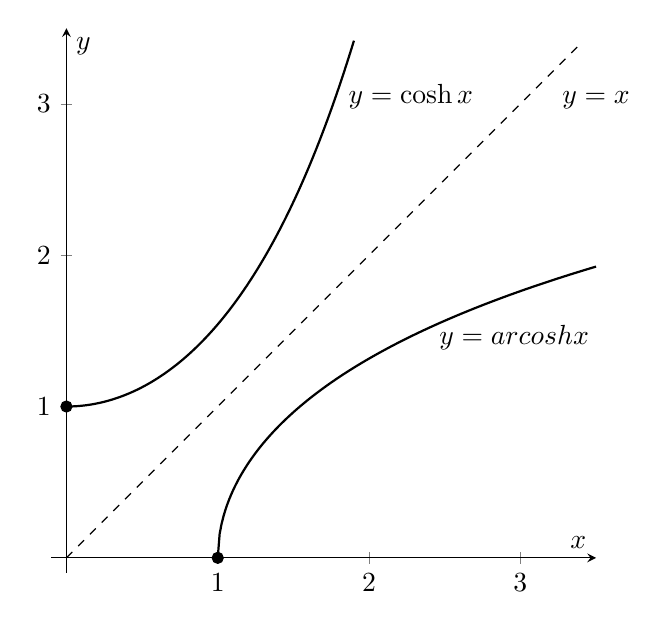
\begin{tikzpicture}
\begin{axis}[
width=8.5cm,
height=8.5cm,
axis lines=middle,
xmin=-0.1, xmax=3.5,
ymin=-0.1, ymax=3.5,
xlabel={$x$},
ylabel={$y$},
xtick={1,2,3},
ytick={1,2,3},
samples=200,
clip=false,
axis equal image
]
\addplot[thick,domain=0:1.9] {(exp(x)+exp(-x))/2};
\addplot[thick,domain=1:3.5] {ln(x + sqrt(x^2 - 1))};
\addplot[dashed,domain=0:3.4] {x};
\addplot[only marks,mark=*] coordinates {(0,1) (1,0)};
\node[above right] at (axis cs:1.8,2.9) {$y=\cosh x$};
\node[below right] at (axis cs:2.4,1.6) {$y=\operatorname{arcosh}x$};
\node[above] at (axis cs:3.5,2.9) {$y=x$};
\end{axis}
\end{tikzpicture}} & & \\
& \msFeature{Shape} & B1 & {Increasing convex curve starting at \((0, 1)\), drawn for \(x \ge 0\) only, labelled.} \\
& \msFeature{Turning points} & B1 & {States the gradient at \(x = 0\) is 0.} \\
& \msFeature{Shape} & B1 & {Increasing concave curve starting at \((1, 0)\), recognisably the reflection of their \(\cosh\) curve in \(y = x\), labelled.} \\
& \msFeature{Symmetry} & B1 & {Equation \(y = x\) stated; the line need not be drawn.} \\
\nopagebreak & & [4] & \\
17(ii) & {\(\left[\sinh x\right]_0^k = \sinh k - \sinh 0\)} & M1 & {Integrates to \(\pm\sinh x\) and substitutes both limits.} \\
& {\(\phantom{\left[\sinh x\right]_0^k} = \sinh k\)} & A1 & \\
\nopagebreak & & [2] & \\
17(iii) & {Reflects in \(y = x\): the two regions together\\[4pt] fill the rectangle \(0 \le x \le \cosh k\), \(0 \le y \le k\)} & M1 & {Relates the two areas, by reflection in \(y = x\), to the rectangle of sides \(k\) and \(\cosh k\); a labelled diagram suffices.} \\
& {\(\int_0^k \cosh x\,\mathrm{d}x\)\\[4pt] \(\phantom{=} + \int_1^{\cosh k} \operatorname{arcosh} x\,\mathrm{d}x = k\cosh k\)} & A1 & {Correct relation oe, such as the \(\operatorname{arcosh}\) integral as \(k\cosh k\) minus the \(\cosh\) integral.} \\
& {\(\text{"}\sinh k\text{"} + \int_1^{\cosh k} \operatorname{arcosh} x\,\mathrm{d}x = k\cosh k\)} & M1 & {Substitutes their result from (ii), of the form \(\pm\sinh k\), into their area relation.} \\
& {\(\int_1^{\cosh k} \operatorname{arcosh} x\,\mathrm{d}x = k\cosh k - \sinh k\)} & A1~AG & {Printed result from a correct area relation and \(\sinh k\), without error. Working backwards from the result earns nothing.} \\
\nopagebreak & & [4] & \\
\nopagebreak \SetCell[c=2]{r} Total for Question 17 & & 10 & \\
\end{msscheme}

\msQuestion{18}
\begin{msscheme}{
  hline{3-6,8-9,11-12,14-18} = {2-Z}{0.4pt, msGrid},
  hline{7,10,13,19} = {0.4pt, msGrid},
  row{19} = {font=\bfseries},
}
Question & Scheme & Marks & Notes \\
18(a) & {\(\frac{2y}{b^2}\frac{\mathrm{d}y}{\mathrm{d}x} - \frac{2x}{a^2} = 0\)} & M1 & {Differentiates implicitly, \(y^2 \to ky\frac{\mathrm{d}y}{\mathrm{d}x}\), or parametrically as \(\frac{\mathrm{d}y}{\mathrm{d}\theta} \div \frac{\mathrm{d}x}{\mathrm{d}\theta}\). Condone coefficient and sign slips.} \\
& {\(\frac{\mathrm{d}y}{\mathrm{d}x} = \frac{b^2x}{a^2y}\)} & A1 & {oe, including \(\frac{b\sinh\theta}{a\cosh\theta}\) parametrically.} \\
& {\(y - b\cosh\theta = \frac{b\sinh\theta}{a\cosh\theta}(x - a\sinh\theta)\)} & M1 & {Substitutes the point into their \(\frac{\mathrm{d}y}{\mathrm{d}x}\) and forms a straight line through \((a\sinh\theta, b\cosh\theta)\) with that gradient.} \\
& {\(ay\cosh\theta - bx\sinh\theta\)\\[4pt] \(\phantom{a} = ab(\cosh^2\theta - \sinh^2\theta) = ab\)} & A1~AG & {Correct substituted tangent equation leading without error, using \(\cosh^2\theta - \sinh^2\theta = 1\), to the printed form.} \\
\nopagebreak & & [4] & \\
18(b) & {\(a\left(\tfrac{b}{a}x\right)\cosh\theta - bx\sinh\theta = ab\)\\[4pt] \(\phantom{a} \Rightarrow x = \ldots\)} & M1 & {Substitutes \(y = \frac{b}{a}x\) (or \(x = \frac{a}{b}y\)) into the tangent and solves for a coordinate.} \\
& {\(P = (ae^\theta,\ be^\theta)\)} & A1 & {oe, such as \(\left(\frac{a}{\cosh\theta - \sinh\theta}, \frac{b}{\cosh\theta - \sinh\theta}\right)\).} \\
\nopagebreak & & [2] & \\
18(c) & {\(y = b \Rightarrow ab\cosh\theta - bx\sinh\theta = ab\)\\[4pt] \(\phantom{a} \Rightarrow x = \ldots\)} & M1 & {Uses \(y = b\) for \(\ell_2\), substitutes into \(\ell_1\) and solves for \(x\). No justification of \(y = b\) needed.} \\
& {\(Q = \left(\frac{a(\cosh\theta - 1)}{\sinh\theta},\ b\right)\)} & A1 & {oe, such as \(x = a\tanh\frac{\theta}{2}\).} \\
\nopagebreak & & [2] & \\
18(d) & {\(x = \tfrac12\left(ae^\theta + \frac{a(\cosh\theta-1)}{\sinh\theta}\right)\)\\[4pt] \(y = \tfrac12(be^\theta + b)\)} & M1 A1 & {\msNote{M1}{Finds the midpoint of their \(P\) and \(Q\), averaging both coordinates.}\\ \msNote{A1}{Both coordinates correct, oe.}} \\
& {\(t = e^\theta\): \(\cosh\theta = \frac{t + t^{-1}}{2},\ \sinh\theta = \frac{t - t^{-1}}{2}\)} & M1 & {Uses exponential definitions to write their midpoint coordinates in terms of \(e^\theta\) alone.} \\
& {\(\frac{\cosh\theta - 1}{\sinh\theta} = \frac{t^2 - 2t + 1}{t^2 - 1} = \frac{t-1}{t+1}\)} & A1 & {oe; implied by a correct \(x\) in \(t\) alone.} \\
& {\(x = \frac{a(t^2+2t-1)}{2(t+1)},\ y = \frac{b}{2}(t+1)\)\\[4pt] \(2ay^2 - 2bxy = 2a\left(\tfrac{b}{2}(t+1)\right)^2\)\\[4pt] \(\phantom{a} - 2b\cdot\frac{a(t^2+2t-1)}{2(t+1)}\cdot\frac{b}{2}(t+1)\)} & dM1 & {Eliminates \(t\): substitutes their \(x\) and \(y\) in \(t\) into \(2ay^2 - 2bxy\), or makes \(t\) the subject of \(y\) and substitutes into \(x\).} \\
& {\(\phantom{a} = \frac{ab^2}{2}\left((t+1)^2 - (t^2+2t-1)\right)\)\\[4pt] \(\phantom{a} = ab^2\)} & A1~AG & {Correct substituted expression or equation leading without error to \(ab^2\), or the printed equation. No comment on the branch needed.} \\
\nopagebreak & & [6] & \\
\nopagebreak \SetCell[c=2]{r} Total for Question 18 & & 14 & \\
\end{msscheme}

\end{document}
